\documentclass[tikz,border=2pt]{standalone}
\usepackage{amsmath}
\usepackage{pgfplots}
\pgfplotsset{compat=1.18}
\begin{document}
% x'(t) = 2t x(t): grey segments have slope f(t,x) = 2tx; the solution from x(0) = 1 is e^{t^2}
% (blue), other solutions are Ce^{t^2} (C = 2, 0.5, -0.5, grey), and x = 0 is the constant solution.
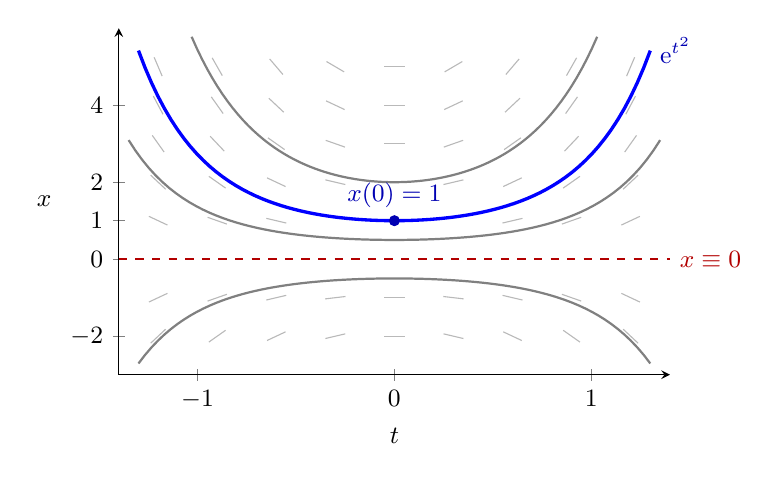
\begin{tikzpicture}[font=\small]
  \begin{axis}[
    axis lines=left, xmin=-1.4, xmax=1.4, ymin=-3, ymax=6,
    xtick={-1,0,1}, ytick={-2,0,1,2,4},
    xlabel={$t$}, ylabel={$x$}, ylabel style={rotate=-90},
    scale only axis, width=7.0cm, height=4.4cm, clip=false, samples=80
    ]
    % slope field: segments of display length 0.26 cm and slope 2tx (1 unit = 2.5 cm in t, 0.489 cm in x)
    \foreach \t in {-1.2,-0.9,...,1.25} {
      \foreach \x in {-2,-1,...,5} {
        \pgfmathsetmacro{\n}{sqrt(2.5^2+(0.489*2*\t*\x)^2)}
        \pgfmathsetmacro{\du}{0.13/\n}
        \pgfmathsetmacro{\dv}{0.13*2*\t*\x/\n}
        \pgfmathtruncatemacro{\keep}{(\x!=0)&&((\x!=1)||(abs(\t)>0.4))}% x = 0 is drawn; room for the label
        \ifnum\keep=1
          \edef\seg{\noexpand\draw[gray!55] (axis cs:\t-\du,\x-\dv) -- (axis cs:\t+\du,\x+\dv);}
          \seg
        \fi
      }
    }
    \addplot[gray, thick, domain=-1.03:1.03] {2*exp(x^2)};
    \addplot[gray, thick, domain=-1.35:1.35] {0.5*exp(x^2)};
    \addplot[gray, thick, domain=-1.3:1.3] {-0.5*exp(x^2)};
    \addplot[red!70!black, thick, dashed, domain=-1.4:1.4] {0};
    \addplot[blue, very thick, domain=-1.3:1.3] {exp(x^2)};
    \fill[blue!70!black] (axis cs:0,1) circle (2pt);
    \node[blue!70!black, anchor=south] at (axis cs:0,1.08) {$x(0)=1$};
    \node[blue!70!black, anchor=west] at (axis cs:1.3,{exp(1.69)}) {$\mathrm{e}^{t^2}$};
    \node[red!70!black, anchor=west] at (axis cs:1.4,0) {$x\equiv0$};
  \end{axis}
\end{tikzpicture}
\end{document}
